\documentclass{dissertation}
%\documentclass[print]{dissertation}
%\documentclass[print,draft]{dissertation}

\hyphenation{TestRoots WatchDog proj-ect proj-ects Ec-lipse two-fold clie-nts Mo-cki-to wide-spread}
\newcommand{\sparkline}[1]{$\vcenter{\hbox{\includegraphics[scale=0.04]{#1}}}$}

\makeglossaries

\newcommand*{\origrightarrow}{}
\let\oldarrow\textrightarrow
\renewcommand*{\textrightarrow}{\fontfamily{cmr}\selectfont\origrightarrow}

% \loadglsentries[main]{glossary}
\newabbreviation{ADL}{ADL}{Activities of Daily Living}
\newabbreviation{ANN}{ANN}{Artificial Neural Network}
\newabbreviation{BA}{BA}{Bundle Adjustment}
\newabbreviation{BCI}{BCI}{Brain-Computer Interface}
\newabbreviation{BMI}{BMI}{Brain-Machine Interface}
\newabbreviation{CAD}{CAD}{Computer-aided Design}
\newabbreviation{CC}{CC}{Constant Curvature}
\newabbreviation{CFA-CON}{CFA-CON}{Closed-Form Approximation of the Coupled Oscillator Network}
\newabbreviation{CFA-UDCON}{CFA-UDCON}{Closed-Form Approximation of the Underdamped Coupled Oscillator Network}
\newabbreviation{CNN}{CNN}{Convolutional Neural Network}
\newabbreviation{Cobot}{Cobot}{Collaborative Robot}
\newabbreviation{COM}{COM}{Center of Mass}
\newabbreviation{CON}{CON}{Coupled Oscillator Network}
\newabbreviation{coRNN}{coRNN}{Coupled Oscillatory Recurrent Neural Network}
\newabbreviation{CS}{CS}{Constant Strain}
\newabbreviation{DCM}{DCM}{Discretized Cosserat Rod Model}
\newabbreviation{DHC}{DHC}{Design Hazardousness Criterion}
\newabbreviation{DMP}{DMP}{Dynamic Motion Primitives}
\newabbreviation{DNN}{DNN}{Deep Neural Network}
\newabbreviation{DOF}{DOF}{Degrees of Freedom}
\newabbreviation{EEG}{EEG}{Electroencephalography}
\newabbreviation{EOM}{EOM}{Equation of Motion}
\newabbreviation{ERD}{ERD}{Event-Related Desynchronization}
\newabbreviation{ERS}{ERS}{Event-Related Synchronization}
\newabbreviation{FEM}{FEM}{Finite Element Method}
\newabbreviation{GAS}{GAS}{Global Asymptotic Stability}
\newabbreviation{GBN}{GBN}{Generalized Binary Noise}
\newabbreviation{GCD}{GCD}{Greatest Common Divisor}
\newabbreviation{GP}{GP}{Gaussian Process}
\newabbreviation{GRU}{GRU}{Gated Recurrent Unit}
\newabbreviation{GVS}{GVS}{Geometric Variable Strain}
\newabbreviation{HCI}{HCI}{Human Computer Interface}
\newabbreviation{HMI}{HMI}{Human Machine Interface}
\newabbreviation{HRI}{HRI}{Human Robot Interface}
\newabbreviation{HNN}{HNN}{Hamiltonian Neural Network}
\newabbreviation{HSA}{HSA}{Handed Shearing Auxetic}
\newabbreviation{ILC}{ILC}{Iterative Learning Control}
\newabbreviation{ISC}{ISC}{Injury Severity Criterion}
\newabbreviation{ISS}{ISS}{Input-to-State Stability}
\newabbreviation{LDA}{LDA}{Linear Discriminant Analysis}
\newabbreviation{LFD}{LFD}{Learning from Demonstration}
\newabbreviation{LNN}{LNN}{Lagrangian Neural Network}
\newabbreviation{LQR}{LQR}{Linear-quadratic Regulator}
\newabbreviation{LSTM}{LSTM}{Long Short-Term Memory}
\newabbreviation{MAE}{MAE}{Mean Absolute Error}
\newabbreviation{ML}{ML}{Machine Learning}
\newabbreviation{MLP}{MLP}{Multilayer Perceptron}
\newabbreviation{MPC}{MPC}{Model Predictive Control}
\newabbreviation{MSE}{MSE}{Mean Squared Error}
\newabbreviation{MSK}{MSK}{Magnet Sensor Kinematics}
\newabbreviation{NN}{NN}{Neural Network}
\newabbreviation{NODE}{NODE}{Neural ODE}
\newabbreviation{ODE}{ODE}{Ordinary Differential Equation}
\newabbreviation{PAC}{PAC}{Piecewise Affine Curvature}
\newabbreviation{PCB}{PCB}{Printed Circuit Board}
\newabbreviation{PCC}{PCC}{Piecewise Constant Curvature}
\newabbreviation{PCS}{PCS}{Piecewise Constant Strain}
\newabbreviation{PDE}{PDE}{Partial Differential Equation}
\newabbreviation{PSNR}{PSNR}{Peak Signal-to-Noise Ratio}
\newabbreviation{ReLU}{ReLU}{Rectified Linear Unit}
\newabbreviation{RL}{RL}{Reinforcement Learning}
\newabbreviation{RMSE}{RMSE}{Root Mean Squared Error}
\newabbreviation{RNN}{RNN}{Recurrent Neural Network}
\newabbreviation{RQ}{RQ}{Research Question}
\newabbreviation{SLAM}{SLAM}{Simultaneous Localization and Mapping}
\newabbreviation{SMP}{SMP}{Stable Motion Primitives}
\newabbreviation{SNN}{SNN}{Spiking Neural Network}
\newabbreviation{SOTA}{SOTA}{State Of The Art}
\newabbreviation{SPCS}{SPCS}{Selective Piecewise Constant Strain}
\newabbreviation{SSIM}{SSIM}{Structural Similarity Index Measure}
\newabbreviation{SVR}{SVR}{Support Vector Regression}
\newabbreviation{VAE}{VAE}{Variational Autoencoder}
\newabbreviation{vSLAM}{vSLAM}{visual SLAM}
\newabbreviation{WMM}{WMM}{World Magnetic Model}


\begin{document}

%% Specify the title and author of the thesis. This information will be used on
%% the title page (in title/title.tex) and in the metadata of the final PDF.
\title{Test Empirical Evaluation of Feedback-Driven Software Development}
\author{Maximilian}{Stölzle}

%% Use Roman numerals for the page numbers of the title pages and table of
%% contents.
\frontmatter

\begin{titlepage}

% \begin{center}
% %% Extra whitespace at the top.
% \vspace*{2\bigskipamount}

% %% Print the title.
% {\makeatletter
% \titlestyle\bfseries\LARGE\@title
% \makeatother}

% %% Print the optional subtitle.
% {\makeatletter
% \ifx\@subtitle\undefined\else
%     \bigskip
%     \titlefont\titleshape\Large\@subtitle
% \fi
% \makeatother}
% \end{center}

\cleardoublepage
\thispagestyle{empty}

\begin{center}

%% The following lines repeat the previous page exactly.

\vspace*{2\bigskipamount}

%% Print the title.
{\makeatletter
\titlestyle\bfseries\LARGE\@title
\makeatother}

%% Print the optional subtitle.
{\makeatletter
\ifx\@subtitle\undefined\else
    \bigskip
    \titlefont\titleshape\Large\@subtitle
\fi
\makeatother}

%% Uncomment the following lines to insert a vertically centered picture into
%% the title page.
%\vfill
%\includegraphics{title}
\vfill

%% Apart from the names and dates, the following text is dictated by the
%% promotieregelement.

{\Large\titlefont\bfseries Dissertation}

\bigskip
\bigskip

for the purpose of obtaining the degree of Doctor

at Delft University of Technology,

by the authority of the Rector Magnificus, Prof.~dr.~ir.~T.H.J.J.~van~der~Hagen,

Chair of the Board of Doctorates,

to be defended publicly on

Monday, 15 September 2025 at 17:30 o’clock

\bigskip
\bigskip

by

\bigskip
\bigskip

%% Print the full name of the author.
\makeatletter
{\Large\titlefont\bfseries\@firstname\ \titleshape{\MakeUppercase{\@lastname}}}
\makeatother

\bigskip
\bigskip

Master of Science ETH in Mechanical Engineering, \\
Swiss Federal Institute of Technology, Switzerland,

born in Göppingen, Germany.

%% Extra whitespace at the bottom.
\vspace*{2\bigskipamount}

\end{center}

\clearpage
\thispagestyle{empty}

%% The following line is dictated by the promotieregelement.
\noindent This dissertation has been approved by the promotors.

%% List the promotors (supervisors).
% \medskip\noindent
% \begin{tabular}{l}
%     Promotor: Prof. Dr.\ R.\ Babu\v{s}ka \\
%     Co-Promotor: Dr.\ C.\ Della Santina
% \end{tabular}

\bigskip
\noindent Composition of the doctoral committee:

%% List the committee members, starting with the Rector Magnificus and the
%% promotor(s) and ending with the reserve members.
\medskip\noindent
\begin{tabular}{p{4.5cm}l}
    Rector Magnificus, & Delft University of Technology, \emph{Chairperson} \\
    Prof.\ Dr.\ R.\ Babu\v{s}ka, & Delft University of Technology, \emph{Promotor} \\
    Dr.\ C.\ Della Santina, & Delft University of Technology, \emph{Co-Promotor} \\

    \medskip
    \mbox{\emph{Independent Members:}} & \\
    Jun.\ Prof.\ Dr.\ G. Rizzello, & Saarland University, Germany\\
    Dr.\ M.\ Bächer, & Disney Research, Switzerland \\
    Prof.\ Dr.\ T.\ A.\ E. Oomen, & Eindhoven University of Technology, Netherlands\\
    Prof.\ Dr.\ G.\ C.\ H.\ E. de Croon, & Delft University of Technology, Netherlands\\
    Prof.\ Dr.\ G. Zardini, & Massachusetts Institute of Technology, USA\\ % & United States of America \\
    Prof.\ Dr.\ Ir.\ M.\ Wisse, & Delft University of Technology, \emph{Reserve member} \\ \\

    % Prof.\ Dr.\ S. Coros, & Swiss Federal Institute of Technology, Switzerland \\
    % % Prof.\ Dr.\ B. Gorissen, & Katholieke Universiteit Leuven, Belgium\\
    % % Prof.\ Dr.\ B. De Schutter, & Delft University of Technology, Netherlands \\
    % Prof.\ Dr.\ G. Chalvatzaki, & TU Darmstadt, Germany \\
    % \multicolumn{2}{l}{Prof. dr. D. Spinellis has contributed to the end phase of writing \ldots} \\
\end{tabular}

%% Include the following disclaimer for committee members who have contributed
%% to this dissertation. Its formulation is again dictated by the
%% promotieregelement.
%\medskip
%\noindent  %Prof.\ Dr.\ D.\ Spinellis has contributed to the creation of this thesis.

% \medskip
% \medskip

\vspace{-1em}

% \medskip
%% Here you can include the logos of any institute that contributed financially
%% to this dissertation.
% \vfill
\begin{center}
    % 
\includegraphics[height=0.5in]{title/logos/tudelft}
    % \hspace{2em}
    % 
\includegraphics[height=0.35in]{title/logos/emerge}\\
    
\includegraphics[height=0.5in]{title/logos/tudelft}
    \hspace{3em}
    \includegraphics[height=0.35in]{title/logos/mit}\\
    \vspace{0.5em}
    
\includegraphics[height=0.3in]{title/logos/emerge}
    \hspace{3em}
    
\includegraphics[height=0.4in]{title/logos/cultuurfonds}
\end{center}
\vfill

\noindent This research was partially funded by the European Union’s Horizon Europe Program from Project EMERGE - Grant Agreement No. 101070918 and by the Dutch Cultuurfonds Wetenschapsbeurzen 2024. The research visit to LIDS/Zardini Lab at MIT was supported by the Rudge (1948) and Nancy Allen Chair.
A significant part of the research appearing in this thesis was developed in collaboration with Prof.\ Dr.\ Daniela Rus and Prof.\ Dr.\ Gioele Zardini from the Massachusetts Institute of Technology, USA.

\noindent Published and distributed by: Maximilian Stölzle. E-mail: \href{mailto:maximilian@stoelzle.ch}{maximilian@stoelzle.ch}\\

\noindent
\begin{tabular}{@{}p{0.2\textwidth}@{}p{0.8\textwidth}}
  \textit{Keywords:} & Soft Robotics, Nonlinear Control, Machine Learning, AI \\[\medskipamount]
      \textit{Printed by:} & Ridderprint | \url{www.ridderprint.nl} \\[\medskipamount]
      \textit{Cover:} & Maximilian Stölzle (Concept) \& Joey Impoza Roberts (Realization) \\[\medskipamount]
      \textit{Style:} & TU Delft House Style, with modifications by Moritz Beller \\[\medskipamount] % \\& \url{https://github.com/Inventitech/phd-thesis-template} \\[\medskipamount]
\end{tabular}

\medskip
\medskip
\noindent All rights reserved. No part of the material protected by this copyright notice may be reproduced or utilized in any form or by any means, electronic or mechanical, including photocopying, recording, or by any information storage and retrieval system, without the written permission of the author.

\vspace{\bigskipamount}

% Copyrighting this is stupid, questionable, and probably illegal, because large parts of the
% thesis have already been published with the copyright resigning with the publisher.
%\noindent Copyright \textcopyright\ 2015 by A.~Einstein

%% Uncomment the following lines if this dissertation is part of the Casimir PhD
%% Series, or a similar research school.
%\medskip
%\noindent Casimir PhD Series, Delft-Leiden 2015-01

%\medskip
\noindent ISBN/EAN: 978-94-6384-836-7\\
\noindent DOI: \href{https://doi.org/10.4233/uuid:24c1f667-8fd6-431a-bb78-11d22f8cb3da}{10.4233/uuid:24c1f667-8fd6-431a-bb78-11d22f8cb3da}

\medskip
\noindent An electronic version of this dissertation is available at \\
\url{http://repository.tudelft.nl/}.

\end{titlepage}



%% The (optional) dedication can be used to thank someone or display a
%% significant quotation.
\dedication{\epigraph{I [...] like to give the maximum in everything I do. The maximum I have. The
    maximum I can give. I am not perfect. But if I do something, I do it [as best I can].
    %And many people are not made like this. There are only few. But I like these few.
  }{Reinhold Messner}}

\tableofcontents

\chapter*{Summary}
\addcontentsline{toc}{chapter}{Summary}
\setheader{Summary}

% Contents of summary:
% \begin{itemize}
%     \item problem and gap (social or scientific relevance) (Introduction)
%     \item thesis aim / main question (Introduction)
%     \item method (Introduction)
%     \item main results (Core chapters)
%     \item conclusion, possible applications, implications
% \end{itemize}

% As we work towards bringing robotics into human-centric environments, safety is paramount. However, today, safety is mostly ensured through computational control policies, which makes it susceptible to perception error and often leads to overly cautious behavior, limiting the robot's performance. Instead, soft robotics promises to improve safety by establishing passive compliance of the entire body through material softness. This \emph{embodied intelligence} is not negatively influenced by perception or control errors. There has been tremendous progress in the last few years in the domain of soft robotics, with new designs, smart materials, actuators, sensors, models, and control approaches being proposed by the research community. In particular, the modeling and control of continuum soft robots is very challenging as they theoretically have infinite degrees of freedom, exhibit complex nonlinear dynamics, and even time-dependent behavior such as hysteresis. Currently, two approaches for control are dominant: model-based control based on physics-based models derived from first principles under significant approximations and learned control policies, mainly by means of reinforcement learning.
% However, there exist major issues with both approaches: i) existing model-based controllers are unable to exploit the full dynamic of soft robots as their underlying models do not sufficiently capture the complex dynamic behavior of soft robots, specifically concerning the influence of actuation and external interaction on the soft robot's deformation, and require expert knowledge in order to meet suitable and appropriate model design choice. On the other side, ii) reinforcement learning does not offer interoperability and stability guarantees and is additionally very sample inefficient, which is an issue when considering the time-dependent material properties and currently limited lifetime of soft robots. 
% Therefore, this thesis argues that a promising alternative approach would be to combine learned models with model-based controllers, which would combine benefits from both worlds: expressive models that require less expert knowledge derived from data combined with controllers whose behavior is interpretable and provably stable.
% The primary challenge for achieving this solution is to identify the necessary characteristics and structures that a learned model needs to exhibit in order to allow us to apply the existing model-based control strategies, such as PID-like feedback+feedforward while making sure that the closed-loop robot system exhibits compliant and safe behavior.
% We tackle this complex challenge in this doctoral thesis through multiple interconnected key contributions:
% 1) leveraging kinematic models for soft robot shape sensing, for example, based on the readout of visual or magnetic sensors, allows us to receive more accurate estimates of the soft robot's state, which is a requirement for effective feedback control; 2) we develop advanced physics-based actuation models, such as modeling the behavior of robots that are actuated through auxetic metamaterials or considering the actuation dynamics of piston-driven pneumatic soft robots;
% 3) we identify techniques that allow us to learn soft robot models with physical structures and stability guarantees. Two of the approaches that we propose are a) an algorithm that identifies low-dimensional, physics-based strain models based on samples of the shape evolution of the robot's backbone and b) a network consisting of coupled harmonic oscillators for learning the latent dynamics of a physical system from high-dimensional observations such as images. The physical structure that is exposed by both approaches allows us to integrate the model into a PID-like feedback controller with potential shaping serving as the feedforward term;
% 4) finally, as a means of moving beyond low-level control, we propose two approaches for generating compliant motion behaviors for soft robots. The first approach, i), is tailored to assist the user, for example, elderly people, with activities of daily living and allows the user to guide the goal of the low-level controller via their thoughts. To achieve a compliant control behavior, we combine motor imagery classified based on the data measured by wearable EEG devices with compliant impedance control in Cartesian space. The second approach, ii) combines an orbitally stable dynamical system in latent space with a bijective neural-network parametrized encoder for learning periodic motions from demonstrations. As the learned motion policy does not rely on a time reference, it allows for natural and compliant tracking of the demonstrated motion.
% The behaviors of some models and controllers have been analyzed theoretically in terms of stability characteristics.
% The models, sensing, control, and motion strategies developed in this thesis have been extensively validated both in simulation and on real-world (soft) robots. The code and data of most chapters have been open-sourced on GitHub.

% As we work towards integrating robotics into human-centric environments, safety remains a paramount concern. While safety is traditionally ensured in rigid robotics through safety-aware computational control policies, this approach is vulnerable to perception errors and often results in overly cautious behavior that limits robot performance. Soft robotics presents a promising alternative by establishing passive compliance throughout the entire robot body through material softness. This mechanical compliance is inherently resistant to perception or control errors. Recent years have witnessed remarkable progress in soft robotics, with researchers developing new designs, smart materials, actuators, sensors, models, and control approaches. However, the modeling and control of continuum soft robots still present significant challenges due to their infinite degrees of freedom, complex nonlinear dynamics, and time-dependent behaviors such as hysteresis. This leads to soft robots that are not sufficiently capable and specifically precise in their motions, making us again sacrifice performance to gain safety. The goal of this thesis is to overcome this tradeoff by combining learned models with efficient model-based control approaches.
As we increasingly strive to integrate robots into human-centric environments, safety is a top priority. Traditionally, rigid collaborative robots have relied on safety-aware computational control policies, which are susceptible to perception errors and often lead to overly cautious behavior that limits performance. In contrast, soft robotics offers a promising alternative by ensuring passive compliance throughout the robot’s structure via material softness. This mechanical compliance inherently mitigates safety issues arising from perception or control errors, although this has been paid with a substantial drop in precision. In recent years, significant advances have been seen in soft robotics, with exciting new developments in design, smart materials, actuators, sensors, models, and control strategies. However, the modeling and control of continuum soft robots continue to pose major challenges due to their infinite degrees of freedom, complex nonlinear dynamics, and time-dependent behaviors like hysteresis. As a result, soft robots often lack the necessary capability and motion precision, leading to a tradeoff where performance is sacrificed for safety. With this thesis, we argue that this tradeoff can be overcome by developing more advanced algorithms that can reason on the physics of the soft robot. More specifically, we propose to overcome this tradeoff by combining powerful learned models with efficient and effective model-based control approaches that allow for interpretability into the actions and admit stability guarantees.

% Currently, two dominant approaches exist for controlling soft robots. The first relies on model-based control using physics-based models derived from first principles under significant approximations. The second directly learns control policies, primarily through reinforcement learning. Both approaches face substantial limitations. Existing model-based controllers cannot fully exploit the dynamics of soft robots as their underlying models inadequately capture complex dynamic behavior, particularly regarding how actuation and external interaction influence the robot's deformation.
% Furthermore, the derivation of these models also requires considerable expert knowledge.
% Finally, the inherent complexity and uncertainty of joined dynamics consisting of the soft robot and its environment make it (currently) infeasible to develop such complex world models from first principles, motivating the need to integrate \gls{ML} approaches that can effectively leverage knowledge contained in data.
% Conversely, directly learning the controller, for example, via reinforcement learning, lacks interpretability into the decision making and stability guarantees while being highly sample inefficient -- a significant drawback given the time-dependent material properties and limited lifetime of current soft robots.
Currently, two main approaches exist for controlling soft robots. The first employs model-based control using approximated physics-based models derived from first principles. The second directly learns control policies, primarily through reinforcement learning. Both strategies face notable limitations. Existing model-based controllers are unable to fully manage and eventually exploit the dynamics of soft robots because their underlying models inadequately capture complex behaviors, particularly how actuation and external interactions affect the robot’s deformation. Moreover, deriving these models requires extensive expert knowledge. Additionally, the combined complexity and uncertainty of the dynamics between a soft robot and its environment make it currently infeasible to develop comprehensive world models from first principles alone, thereby motivating the integration of \gls{ML} approaches that can effectively leverage data-driven insights. Conversely, directly learning the controller — such as via reinforcement learning — lacks interpretability and stability guarantees while being highly sample inefficient, a significant drawback given the time-dependent material properties and limited lifespan of current soft robots.

% The primary challenge lies in identifying the necessary characteristics and structures that a learned model must possess to enable the application of existing closed-form model-based control strategies, such as PID+potential-shaping while ensuring the closed-loop robot system maintains compliant, stable, and safe behavior.

% With this thesis, we argue that combining learned models with model-based controllers offers a promising alternative approach, uniting the benefits of both methods: expressive models derived from data requiring less expert knowledge coupled with controllers whose behavior is both interpretable and provably stable. 
% While in recent years, there has been increased research interest in leveraging learned models for control, most works rely on computationally demanding optimal control approaches, such as \gls{MPC}, to optimize the actuation sequence. However, the computational complexity of solving this optimal control problem limits the maximum control rate during deployment not allowing us to exploit the dynamic capabilities of soft robots fully.
% Instead, we pursue in this thesis closed-form controllers that leverage the physical structure of learned models within an energy-shaping feedforward term.
% The primary challenge here lies in devising approaches for incorporating such physical structures (specifically kinetic and potential energy terms) into the learning of dynamical models of soft robots.
In this thesis, we contend that combining learned models with model-based controllers presents a promising alternative that brings together the advantages of both approaches: expressive, data-driven models that require less expert knowledge paired with controllers that are both interpretable and provably stable. Although recent years have seen increased interest in leveraging learned models for control, most work in this area depends on computationally intensive optimal control methods, such as \gls{MPC}, to optimize the actuation sequence with the learned model. However, the high computational cost of solving these optimal control problems limits the maximum control frequency during deployment, preventing us from fully exploiting the dynamic capabilities of soft robots. Instead, this thesis pursues closed-form controllers that utilize the physical structure of learned models within an energy-shaping feedforward term. The main challenge here is to develop approaches that integrate such physical structures—specifically, kinetic and potential energy terms—into the learning of dynamical models for soft robots.
% Before we could tackle this main challenge, we first had to advance physics-based models derived from first principles and identify new techniques to exploit them for control. On one hand, this informed us about the physical priors that we have access to for learning and on the other hand it inspired us how we can leverage model-based controllers with learned models.
Before addressing this main challenge, we first had to advance physics-based models derived from first principles and identify novel techniques to leverage them for control. On one hand, this clarified which physical priors were available for learning, while on the other hand, it inspired new ways to integrate model-based controllers with learned models.
The thesis addresses this topic through several interconnected key contributions. 

First, we argue that quantifying the safety of soft robots is crucial for designing and controlling them to ensure that the closed-loop system meets the specific safety requirements of their intended applications. To this end, we present the first safety metric for continuum soft robots, which assesses the safety of an integrated soft robot design by accounting for both its embodied and computational intelligence.

% Secondly, this thesis advances kinematic models for soft robot shape sensing, utilizing visual or magnetic sensor readings to obtain more accurate estimates of the soft robot's state—a crucial requirement for effective feedback control.
% Secondly, this thesis improves shape sensing for soft robots by leveraging kinematic model knowledge. We achieve this by formulating and solving nonlinear optimization problems that reconcile sensor measurements with the attainable backbone shapes by the kinematic model.
% We develop two distinctive approaches that combine commercial sensors, specifically visual and magnetic sensors, with a \gls{SLAM} algorithms and a learned sensor measurement model, respectively, to estimate the soft robot's state—a crucial requirement for effective feedback control.
Secondly, this thesis enhances shape sensing for soft robots by leveraging insights from kinematic models. We accomplish this by formulating and solving nonlinear optimization problems that align sensor measurements with the backbone shapes predicted by the kinematic model. We present two distinct approaches that integrate commercial sensors—namely visual and magnetic—with SLAM algorithms and a learned sensor measurement model, respectively, to accurately estimate the soft robot’s state, a key requirement for effective feedback control.

% Thirdly, the thesis develops sophisticated physics-based actuation models, including those for robots actuated through auxetic metamaterials, called \gls{HSA} robots, and models accounting for the actuation dynamics of piston-driven pneumatic soft robots. Subsequently, we exploit the gained model knowledge within provably stable nonlinear controllers - namely, an integral-saturated PID+potential shaping and Cartesian-space impedance control for planar \gls{HSA} robots and a backstepping controller for pneumatic piston-driven soft robots.
% This contribution highlights the control-oriented structure of physics-based models, which will be utilized in the subsequent contribution. Additionally, the research underpinning this contribution reveals the current limitations regarding the complexity and computational demands of physics-based models, thereby motivating the exploration of potentially more computationally efficient neural network-parametrized models.
% This contribution improves our understanding of an essential ingredient of soft robot behavior - the actuation - and demonstrates how such knowledge can be leveraged within model-based control approaches.
% Furthermore, the work with \gls{HSA} robots demonstrated some of the limitations of fully physics-based models at capturing very complex characteristics such as hysteresis, motivating the exploration of learning-based approaches. In the future, the actuation models developed as part of this contribution can serve as strong physical priors for learned models.
Thirdly, this thesis introduces advanced physics-based actuation models, including those for robots actuated by auxetic metamaterials —- referred to as \gls{HSA} robots—and models that capture the actuation dynamics of piston-driven pneumatic soft robots. We then leverage the acquired model insights to design provably stable nonlinear controllers—specifically, an integral-saturated PID combined with potential shaping and Cartesian-space impedance control for planar \gls{HSA} robots, as well as a backstepping controller for pneumatic piston-driven soft robots. This contribution deepens our understanding of actuation, a critical aspect of soft robot behavior, and demonstrates how such insights can be incorporated into model-based control strategies. Moreover, experiments with \gls{HSA} robots have highlighted the limitations of purely physics-based models in capturing complex phenomena like hysteresis, thereby motivating the exploration of learning-based approaches. In the future, the developed actuation models can serve as valuable physical priors for learned models.

% Fourthly, the thesis identifies techniques for learning soft robot models with physical structures and stability guarantees. 
% We achieve this by integrating physics-based dynamical models into the learning algorithm which determines the free parameters of the dynamics and optimally optimizes over a change of coordinates, such as an encoding into latent space.
% Two notable approaches are presented: (1) an algorithm that identifies low-dimensional, soft robot strain models using samples of the robot backbone's shape evolution and (2) a network of coupled harmonic oscillators for learning latent dynamics of physical systems from high-dimensional observations such as images. 
% The kinematic and potential energy terms of the learned models allow for stability analysis using standard tools from nonlinear system theory (e.g., Lyapunov arguments).
% For example, we prove that the presented coupled oscillator network is globally asymptotically stable and input-to-state stable.
Fourthly, the thesis presents techniques for learning soft robot models that incorporate physical structures while ensuring stability. We accomplish this by embedding physics-based dynamical models into the learning algorithm, which determines the free parameters of the dynamics and optionally optimizes a coordinate transformation—such as encoding into latent space. Two notable approaches are introduced: (1) an algorithm that extracts low-dimensional soft robot strain models from samples of the robot backbone’s shape evolution, and (2) a network of coupled harmonic oscillators for learning latent dynamics from high-dimensional observations like images. The explicit inclusion of kinematic and potential energy terms in these models allows for stability analysis using standard nonlinear system theory tools, such as Lyapunov methods. For instance, we prove that the coupled oscillator network is both globally asymptotically stable and input-to-state stable.

% The physical structure exposed by both approaches enables their integration into PID-like feedback controllers with potential shaping as the feedforward term.
% Fifthly, we leverage the physical structure of the learned models from contribution four to devise closed-form setpoint regulators. The controller consists of (1) a potential shaping feedforward term that ensures that the local/global minimum of the potential energy is at the setpoint leveraging the learned model knowledge and (2) an integral-saturated PID as the feedback term for rejecting disturbances and counteracting modeling errors preventing steady-state errors.
% The stability of the closed-loop system can be again analyzed using Lyapunov methods.
Fifthly, we exploit the physical structure of the learned models from contribution four to design closed-form setpoint regulators. The controller contains two key components: (1) a potential shaping feedforward term that positions the local/global minimum of the closed-loop potential energy at the setpoint by leveraging the learned model knowledge, and (2) an integral-saturated PID feedback term that rejects disturbances and compensates for modeling errors to prevent steady-state errors. The stability of the closed-loop system can then be analyzed using Lyapunov arguments.


Finally, the thesis explores methods for generating compliant motion behaviors in soft robots beyond low-level control. One approach focuses on assisting users, particularly elderly individuals, with activities of daily living by guiding the low-level controller with brain signals. This is achieved by combining motor imagery classification from wearable EEG devices with compliant impedance control in operational space. The second approach combines an orbitally stable dynamical system in latent space with a bijective neural network parametrized encoder to learn periodic motions from demonstrations. By avoiding reliance on time references, this learned motion policy enables natural and compliant tracking of demonstrated periodic motions. This contribution ensures that not just the robot structure and low-level controller are compliant but also the high-level motion strategy.

% The thesis includes a theoretical analysis of the stability characteristics of several models and controllers. All proposed models, sensing methods, control strategies, and motion approaches have undergone extensive validation through either simulation or real-world testing on soft robots. Additionally, the code and data from most chapters have been made publicly available through GitHub, contributing to the broader research community's ongoing work in this field.


% Conclusion about the core contribution:
% \begin{itemize}
%     \item Goal of this thesis: safe and precise soft robot behavior. Safety is increase by the soft body and learned models can more accurately capture complex dynamics, leading to hopefully increased precision in the future.
%     \item In summary, we proposed strategies for learning dynamics that... and that allow for closed-form model-based control, which is computationally very efficient. 
%     \item Verified in simulation and code is available online
%     \item Limitations include lack of experimental validation, focus on setpoint regulation, no underactuated setting, no environment interactions, no explicit accounting for safety in control
% \end{itemize}

% In summary, the goal of this thesis is to work towards safe and precise soft robot behavior in human-centric environments.
% Here, the safety is contributed by the soft body with its mechancial compliance (both on a structural and surface level).
% To increase the precision of soft robots while preserving insight into the decision-making, stability guarantees, and computational efficiency, the thesis's core contribution is the development of closed-form soft robot controllers based on learned models. Specifically, we propose to leverage the physical structure of learned models within a setpoint regulation controller consisting of an integral-saturated PID as the feedback term and a potential shaping feedforward term.
% To enable this, we developed two \gls{ML} approaches which allow us to express the kinetic and potential energy of the learned dynamics.
% Several contributions support this core contribution, such as a metric to quantify the safety of soft robots, strategies for integrating kinematic models into shape sensing approaches, advanced physics-based actuation models which can serve in the future as additional priors on the learned models, and moving one level above low-level control compliant motion generation strategies for soft robots.
% All proposed models, sensing methods, control strategies, and motion approaches have undergone extensive validation through either simulation or real-world testing on soft robots.
% The code and data from most chapters have been made publicly available on GitHub, contributing to the broader research community's ongoing work in this field.
% Limitations of the core contribution include a lack of experimental validation of the model learning and the control with learned models, that the trajectory tracking and underactuated settings are currently not considered, that the model learning does not (explicitly) account for environment interactions, and that the proposed controller does not directly consider the safety of the closed-loop system (i.e., the controller is not safety-aware)
In summary, this thesis aims to work towards safe and precise soft robot behavior in human-centric environments. In this context, safety is achieved through the soft body’s mechanical compliance. To enhance precision while maintaining insight into decision-making, ensuring stability, and preserving computational efficiency, the core contribution of this work is the development of closed-form soft robot controller architectures and their connection to learned models. 
% Specifically, we propose leveraging the physical structure inherent in these learned models within a setpoint regulation controller that combines an integral-saturated PID feedback term with a potential shaping feedforward term. To facilitate this, we developed two \gls{ML} approaches that enable us to express the kinetic and potential energy of the learned dynamics. 
Several supporting contributions include a metric for quantifying the safety of soft robots, strategies for integrating kinematic models into shape sensing methods, advanced physics-based actuation models that could serve as future priors for learned models, and moving beyond low-level controllers by devising compliant motion strategies. All proposed models, sensing methods, control strategies, and motion approaches have been thoroughly verified through simulation or real-world testing on soft robots. The code and data from most chapters have been made publicly available on GitHub, thereby contributing to the broader research community. 

%Limitations of the core contribution include a lack of experimental validation for both the model learning and the control with learned models, the current omission of trajectory tracking and underactuated scenarios, the fact that the model learning does not explicitly account for environmental interactions and that the proposed controller does not explicitly consider the safety of the closed-loop system.



% \chapter*{Samenvatting}
% \addcontentsline{toc}{chapter}{Samenvatting}
% \setheader{Samenvatting}

% {\selectlanguage{dutch}

%   Samenvatting in het Nederlands.
% }

% \chapter*{Zusammenfassung}
% \addcontentsline{toc}{chapter}{Zusammenfassung}
% \setheader{Zusammenfassung}

% {\selectlanguage{german}

%   Zusammenfassung in Deutsch.
% }




\chapter*{Acknowledgments}
\addcontentsline{toc}{chapter}{Acknowledgments}
\setheader{Acknowledgments}

% First of all and most importantly, thank you to my advisor and co-promotor Dr. Cosimo Della Santina for taking a chance on me and giving me this opportunity to pursue a Ph.D., for at start giving me a very well defined and well guided research project that allowed me to get acquinted with soft robotics and advanced nonlinear control theory in a rapid, step-by-step fashion with a significantly flattened learning curve, for always spot-on technical guidance whenever I had questions or encountered technical difficulties, the always candid but highly constructive and feedback on research and paper drafts - serving as the ''\emph{feared}`` \emph{\nth{2}}-reviewer already long before paper submission, for all the advice in structuring slides which allowed me to significantly elevate my presentation skills, for already early on trusting me in contributing to student mentoring, for giving me the connections and platforms to pursue impactful collaborations on a European and international level, for gradually allowing me to work more independently and propose research projects and manage projects myself, for gradually giving me more ''senior``reponsibilities such as leading the development of the ICS PA and EU EMERGE deliverables, and most importantly for consistently and effectively supporting me through the entire Ph.D. journey.
First and foremost, I want to thank my advisor and co-promotor, Dr. Cosimo Della Santina, for believing in me and giving me the chance to pursue a Ph.D. Initially, you entrusted me with a well-scaffolded project that let me dive into soft robotics and advanced nonlinear control step by step, smoothing the learning curve. Over time, you progressively empowered me to design and manage research projects on my own. Your technical guidance was always spot-on whenever I hit a roadblock, and your candid yet constructive feedback on my research and draft papers—serving as the ''feared second reviewer`` long before paper submission—pushed the work to a higher standard. Your coaching on presentation structure and slide style elevated my presentation skills, and your early confidence in my ability to mentor students broadened my professional growth. Thank you for connecting me with leading collaborators across Europe and beyond, and for gradually entrusting me with \emph{senior} responsibilities like leading the ICS practical assignment and EU EMERGE deliverables. Above all, thank you for your steadfast and effective support throughout this entire Ph.D. journey.

I am deeply grateful to my advisor, Professor Robert Babuška, for always being available and for responding so quickly to every request. His critical assessments of my progress, streamlined coordination, fast feedback on thesis drafts, and our engaging discussions about the propositions were invaluable.

Professors Daniela Rus and Gioele Zardini, the many impactful collaborations with you fundamentally shaped this Ph.D. research, and my visiting period in your groups significantly contributed to my personal development—thank you.

I appreciate the independent committee members—Junior Professor Gianluca Rizzello, Dr. Moritz Bächer, Professors Tom Ooomen, Guido de Croon, and Gioele Zardini—for graciously accepting the invitation, accommodating our scheduling constraints, and dedicating significant time to reviewing the thesis and attending the defense.

I am indebted to all scientific collaborators whose contributions enliven the chapters of this thesis. In particular, Ryan Truby and Lillian Chin, thank you for inviting me to work on the HSA robot platform—a project that was both enjoyable and pivotal to this thesis.
Thank you, Sonal Baberwal, for a highly interdisciplinary and almost daring collaboration on brain-controlled soft robots—bold, harmonious, and ultimately very successful. Working on this project with you was a joy, and I’m grateful for the friendship we’ve built along the way.

Thank you to all my students—whether you joined for a research internship, a Bachelor End Project (BEP), or a master’s thesis—for trusting my project ideas and guidance. Your motivation, dedication, and creativity made our work both productive and inspiring, and many of your projects became publications that form the backbone of this dissertation.
I had the privilege of co-mentoring several M.S. students—Emanuele Rosi, Ricardo Valadas, Gabriele Di Marzo, Riccardo Sepe, Gioele Buriani, and Iván López Brocéno—as well as the 2023 BEP team of Bendert de Roij van Zuidewijn, Hannah Gielen, Quirijn Bos, and Floris Cuperus.
A special shout-out goes to the 2021 BEP team—Thomas Baaij, Marn Klein Holkenborg, Daan van der Tuin, and Jonathan Naaktgeboren. From my first month as a Ph.D. student, I had the privilege to be involved in your BEP project, which subsequently inspired an ambitious research project that you embraced, even though it was (initially) well beyond the techniques you knew at the time. Your perseverance over the 1.5 years turned that idea into a joint publication, and our collaboration was filled with unforgettable moments—not least your ''Lord of the Rings``-inspired animation of our journey together.

My master’s mentors at ETH Zürich—Julian Zilly (IDSC), Takahiro Miki (RSL), Martin Azkarate and Levin Gerdes (PRL @ ESA), Florian Achermann, Nicholas Lawrance, and Jen Jen Chung (ASL)—ignited my passion for robotics and helped me build the foundation that made this Ph.D. possible.

Beginning in the CoR department during COVID, when on-site work was limited to one day a week, was unusual. I am especially grateful to department veterans Bruno Brito and Padmaja Kulkarni, and at the time senior master student Francesco Stella, for their warm welcome.
Shortly after I began my Ph.D., postdocs Pablo Borja and Sagar Joshi joined the group. Thank you both for fostering a friendly lab culture and for the many enjoyable dinners and drinks we shared.
To the PhI-Lab teammates who joined later—Pietro Pustina, Tomás Coleman, Anton Bredenbeck, Jiatao Ding, Chuhan Zhang, Jingyue Liu, Ebrahim Shahabi, Giovanni Franzeso, Rodrigo Pérez-Dattari, Zhaoting Li, Mariano Ramirez Montero, Daniel Feliu Talegon, Kirsten Lussenburg, and Semanur Küçük—thank you for the great times and for our successful collaborations on research, the ICS course, and student mentoring.

I also appreciate our visiting researchers—Kyle Walker, Xiang-Yu Shao, Maja Trumić, Francesco Piqué, Michele Pierallini (a fantastic Pisa tour guide), Sonal Baberwal (an exceptionally kind collaborator), Domenico Donà, Michele Martini, and Lorenzo Paiola—for bringing fresh perspectives and for the memorable moments we shared.

Special thanks to Pietro Pustina for always being ready to help whenever I (yet again) had a question about control theory or actuation coordinates.

To my TUD-EMERGE teammates Jingyue Liu, Mariano Ramirez Montero, and Ebrahim Shahabi: thank you for your effective teamwork on our many time-consuming reports and deliverables. I also thank the entire EMERGE consortium for our productive collaboration on cutting-edge interdisciplinary topics—especially our Pisa partners Andrea Ceni, Andrea Cossu, Claudio Gallichio, and Davide Bacciu.

I’m grateful to all past and present CoR colleagues for making the department such a supportive place, cultivating a spirit of collaboration, and always being willing to lend expertise or equipment. Bas van der Heijden, Giovanni Franzeso, Rodrigo Pérez-Dattari, and Lasse Peters—thank you for the many insightful research discussions.
My sincere thanks go as well to the CoR secretaries for their kindness, assistance, and for shielding us from excessive university bureaucracy.

My time at MIT was truly transformative. I thank Daniela Rus and Gioele Zardini for making the visit possible, and my many peers—Zach Patterson, Konstantin Rusch, Annan Zhang, Erfan Aasi, Emily Sologuren, Pascal Spino, Joseph DelPreto, Alaa Maalouf, Shiva Sreeram, Wei Xiao, Kiwan Wong, Xinling Li, Yujun Huang, Jiarui Li, Marius Furter, and Riccardo Fiorista—for their warm welcome and for including me in every group activity. I am especially grateful to Konstantin Rusch and Zach Patterson for their impactful collaboration and effective mentorship, and to Kiwan Wong for trusting my guidance—despite initial reluctance to revisit soft-robot projects.
Although my Boston schedule was hectic, the experiences and time spent with friends were essential to maintaining a healthy work-life balance. Among many others, thank you, Niccolò Pagliarani, Francesco Stella, Laurence Willemet, Luzia Knödler, Alberto Comoretto, Viola Del Bono, and Deniz Albayrak for the memorable gatherings, dinners, parties, and good times.

Organizing the Priors4Robots workshop at RSS 2024 was both insightful and fun. I thank all co-organizers—especially John Alora, Luis Pabon, and Roshan Kaundinya—for the great camaraderie (and I’m sorry I couldn’t guide you around Delft in person). I also appreciate every speaker who accepted our invitation, and Michael Lutter for the fascinating private tour of Boston Dynamics.

Conferences and Ph.D. schools were among the most enjoyable parts of my doctoral journey, offering the chance to meet researchers in related fields and build lasting friendships. Niccolò Pagliarani, Burcu Seyidoglu, Francesco Stella, Brandon Caasenbrood, Nana Obayashi, Kai Junge, Zach Patterson, Annan Zhang, Lillian Chin, Ian Good, Davide Calzolari, Mariano Ramirez Montero, Daniel Feliu Talegon, and many others: thank you for the unforgettable RoboSoft adventures and the connected trips to Bali, Joshua Tree National Park, Los Angeles, Portofino, and beyond.
My thanks go to the Dutch soft-robotics community for organizing outstanding symposia and Ph.D. schools, and especially to Brandon Caasenbrood, Philip Mitterbach, Benn Proper, Krishna Kommuri, Mostafa Atalla, Nick Willemstein, and Vera Kortman for the great experiences. It was a pleasure meeting Enrico Donato, Niccolò Pagliarani, Burcu Seyidoglu, Elisa Setti, and many others at the Dutch Soft-Robotics Summer School—thank you all.
Enrico Donato, Elisa Setti, Philip Mitterbach, Benn Proper, Michele Martini, Pietro Pustina, and Daniele Caradonna—thank you for the exceptional culinary adventures in Rome during the soft-robotics modeling and control graduate course.
Despite occasionally feeling like an outsider in the control-systems community, the mostly DLR crew—Davide Calzolari, George Pollayil, and Xuming Meng—made ACC 2022 in Atlanta a blast. ISER 2023 in Chiang Mai was equally enjoyable, thanks to Christopher Bradley, Adrian Piedra, Rafael Papallas, and Nathaniel Simon. 
Mónika Farsang, thank you for teaming up at DRL and for navigating the kilometer-long row of posters with me at NeurIPS 2024 in Vancouver.

To my colleagues and friends in Delft: you made this period special and joyful. Many of my original office mates—Luzia Knödler, Elia Trevision, Yujie Tang, Anna Mészáros, Saray Baker, Khaled Mustafa, and Nils Wilde—started around the same time I did, and together we navigated the highs and lows of Ph.D. and research life. I cherished our lunch-time conversations, tea breaks, and social outings—dinners, karting, skiing, bouldering, tennis, and more. Julian Schumann, thank you for supplying so many delicious cakes for our ''cake breaks`` and for the fun tennis matches.
Tomás Coleman, Anton Bredenbeck, and Italo Belli—thank you for hosting countless barbecues and dinners that united the department. I also appreciate the many other wonderful people at CoR—Corrado Pezzato, Giovanni Franzese, Rodrigo Pérez-Dattari, Mariano Ramirez Montero, Gustavo Rezende, Alvaro Serra Gómez, Jelle Luijkx, Julian Schumann, Max Lodel, Oscar de Groot, Andreu Matoses Gimenez, Max Spahn, Lorenzo Lyons, Dennis Benders, Anastasios (Tasos) Tsolakis, Linda van der Spaan, Bas van der Heijden, Bruno Brito, Alex Ratschat, Ekaterina (Katy) Karmanova, and Fiorella Sibona—for cultivating such a positive department atmosphere.

My social support system has been vital—lifting my spirits, providing welcome distractions from research stress, and accepting the time demands of a Ph.D. I thank my Swiss friends Loris, Philip, Laurens, Daniele, and Claudio for always making me feel at home when I visited. I’m sorry the Netherlands and its beach bars didn’t fully win you over a few years ago; I hope your visit for my defense changes that.

Above all, I am deeply grateful to my family—especially my mom, Sabine, and my brother, Johannes—for being the rock I can always lean on and for inspiring me to become the best version of myself.

To my life partner over this period, Léa: thank you for sharing these years with me and for the many sacrifices you’ve made—most notably moving to Delft / the Netherlands, to join me on this journey. I appreciate your understanding of the long workdays, weekend hours, deadline-driven vacation schedules, and the period abroad in the US that were part of this Ph.D. Your unwavering love and belief in me have been an incredible source of strength and support.

I’m sure I have inadvertently overlooked others who made meaningful contributions to this Ph.D. journey—please know you have my deepest thanks as well.


\section*{Acknowledgements Relating to Specific Chapters}
\vspace{0.3cm}

\begin{itemize}
    \item \textbf{Samenvatting} I would like to thank Saray Bakker for proofreading and revising the Dutch translation of the thesis summary.
    \item \textbf{Chapter~\ref{chp:hsamodel}.} The authors would like to thank Ian Good and Jeffrey Lipton from the University of Washington, U.S., for sharing the mechanical characterization published in \citep{good2022expanding}. We also acknowledge Sagar Joshi from the Delft University of Technology, the Netherlands, for their valuable guidance on attaching reflective markers to the HSA.
    \item \textbf{Chapter~\ref{chp:hsacontrol}.} We would like to acknowledge Pietro Pustina for the valuable insights into a coordinate transformation into collocated variables, control of underactuated soft robots, and his help in revising Chapter~\ref{chp:hsacontrol}.
    \item \textbf{Chapter~\ref{chp:braincontrol}.} The authors thank Dr. Fabien Lotte for his suggestions concerning the protocol, Dr. Tomas Ward and the Neuroconcise team for their support with the FlexEEG device, and J.K. Balasubramanian for his assistance with the EEG setup.
    \item \textbf{Chapter~\ref{chp:promasens}.} The authors acknowledge Ehsan Hoseini, Jasper Insinger, and Tom Salden from Delft University of Technology, the Netherlands, for their guidance in designing the \gls{PCB}.
    \item \textbf{Appendix~\ref{chp:apx:holisticcodesign}.} The authors would like to acknowledge Yujun Huang and Marius Furter from the Zardini Lab at MIT and Andrew Fletcher from UC San Diego for reviewing the manuscript draft.
\end{itemize}

\begin{flushright}
{\makeatletter\itshape
    Maximilian Stölzle \\
    Delft, August 2025
\makeatother}
\end{flushright}




%% Use Arabic numerals for the page numbers of the chapters.
\mainmatter

%% Turn on thumb indices.
\thumbtrue

\chapter{Introduction}
\label{introduction}

\begin{abstract}
Sample Abstract.
\end{abstract}

\blfootnote{This chapter is partly based on \faFileTextO~\emph{M. Beller. Toward an
    Empirical Theory of Feedback-Driven Development, ICSE'18 (Student Research Competition)}~\cite{BellerSRC2018}.
}


\newpage

\dropcap{T}his is a introductory page.

\section{Background \& Context}
% In this thesis, you can reference pictures~\Cref{fig:devmodel} using Cleverref and circles \circled{5}.

% \begin{figure}[htb]
% 	\centering
% 	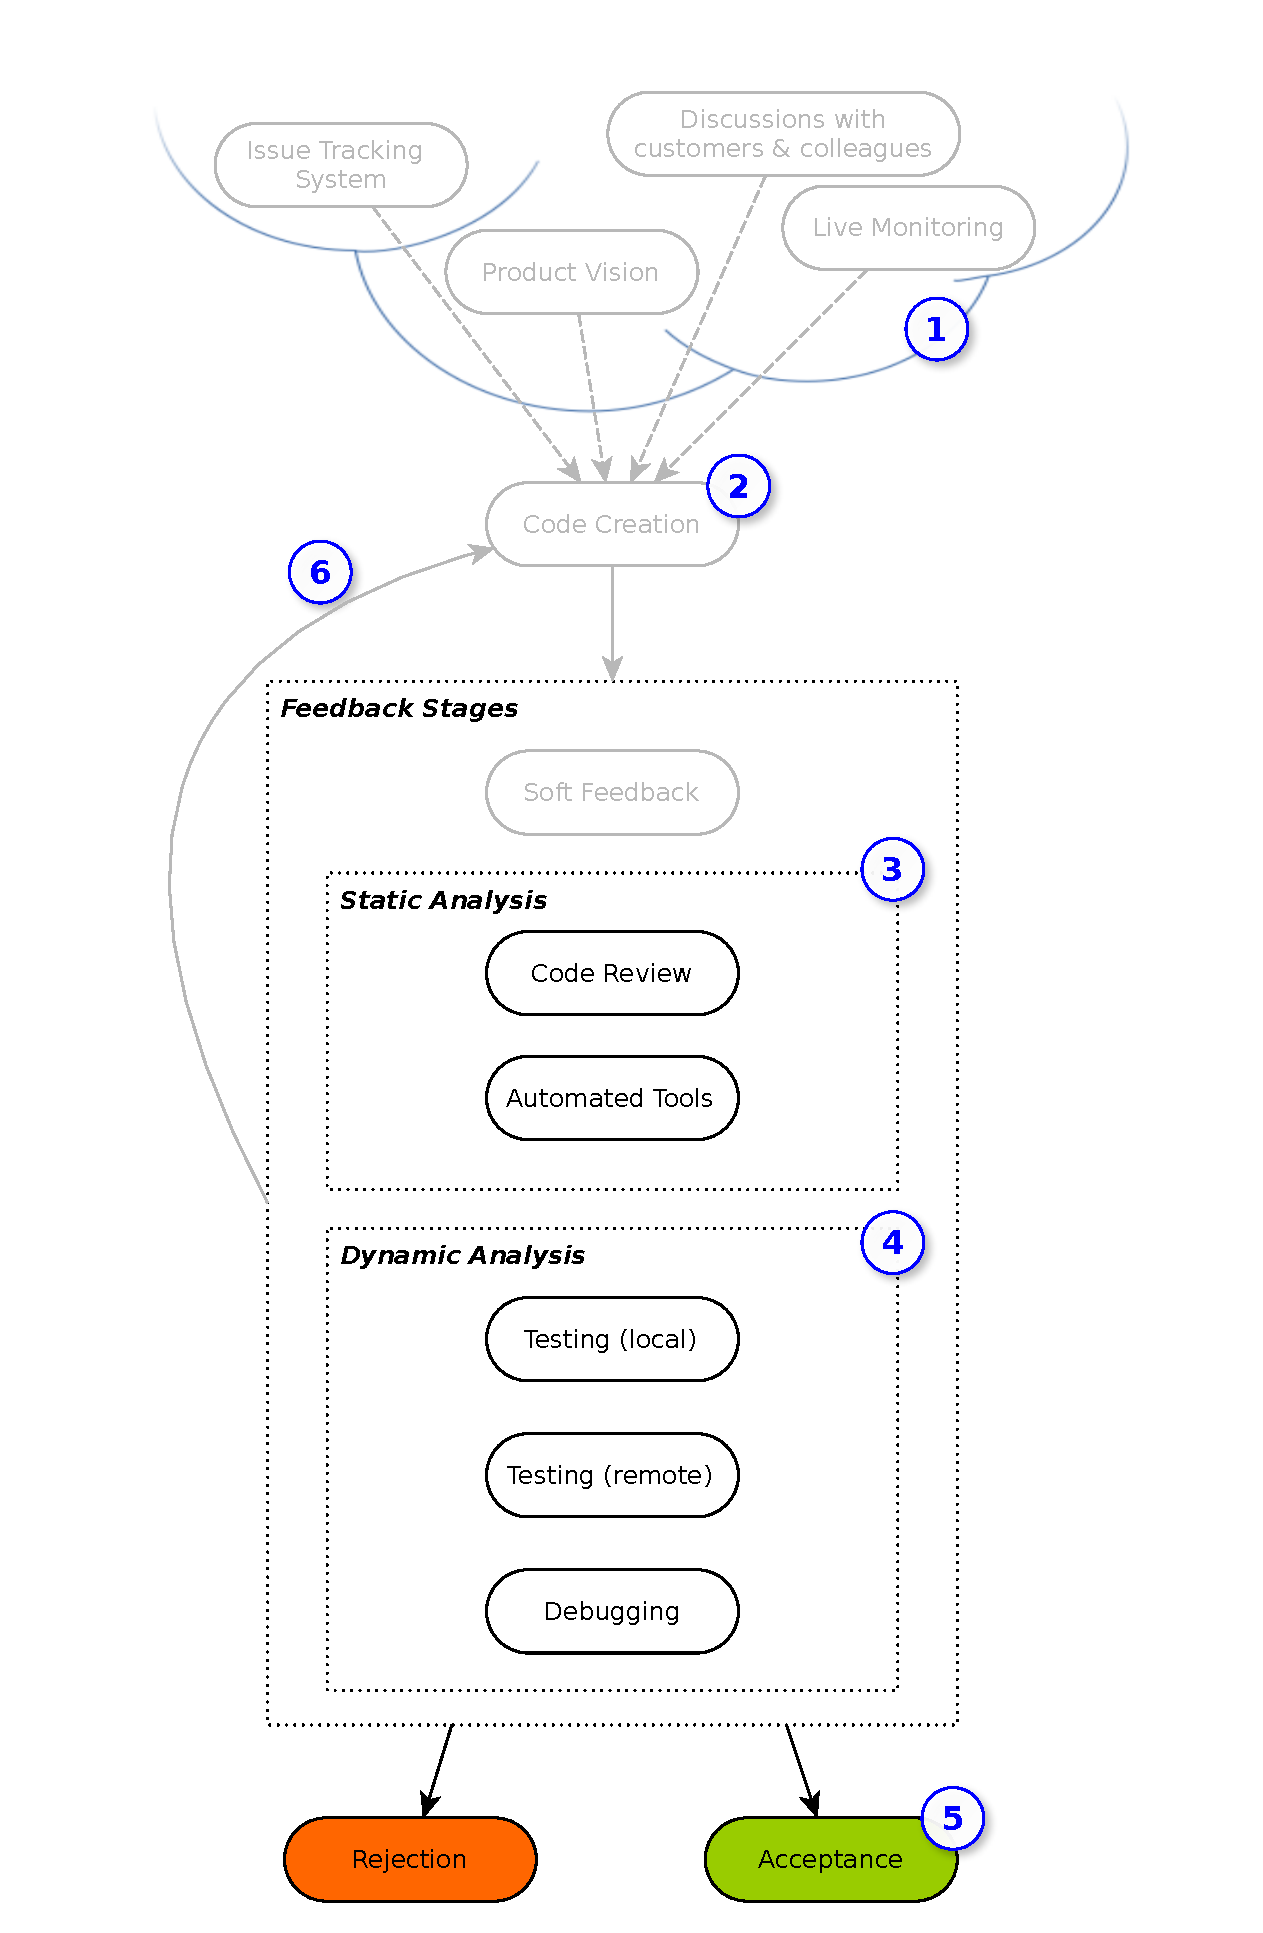
\includegraphics[width=0.65\columnwidth]{development_model_without_papers}
% 	\caption{The stages of the FDD model and their relationship to other
%           Software Engineering concepts.}
% 	\label{fig:devmodel}
% \end{figure}

We also have lists:

\begin{enumerate}
  \item Static Analysis~\circled{3} examines program artifacts or
    their source code without executing them~\cite{wichmann1995industrial}, while
 \item Dynamic Analysis~\circled{4} relies on information gathered from their
   execution~\cite{cornelissen2009systematic}.
\end{enumerate}

Or boxes:

\begin{framed}
This thesis is concerned with the empirical assessment of the state of the art of how developers
drive software development with the help of feedback loops. \cite{boyer2020dynamics}
\end{framed}

Or code:
\begin{lstlisting}[caption={\textsc{TrinityCore}},label={lst:e1}]
 x += other.x;
 y += other.y;
 z += other.y;
\end{lstlisting}


I hope this helps you get started!
Moritz

First time should be long: \gls{GCD}
Next time should be short: \gls{GCD}

\chapter{Conclusions and Future Work}
\label{chp:conclusion}
% Write a separate chapter called ‘Conclusion’ (or, for example, Conclusion & Discussion)
% - Present a clear answer to your main question / relate conclusions clearly to your main aim
% - Evaluate the validity of that answer in light of possible limitations
% - State the scientific and societal importance of your study
% - Reflect on possible applications and suggest avenues for future research

The conclusions of your thesis.

\section{Conclusions}\label{sec:conclusions}

\section{Future Work}\label{sec:future_work}


%% Use letters for the chapter numbers of the appendices.
%\appendix

%\include{appendix-a/appendix-a}

%% Turn off thumb indices for unnumbered chapters.
\thumbfalse

\chapter*{Bibliography}
\addcontentsline{toc}{chapter}{Bibliography}
\setheader{Bibliography}

URLs in this thesis have been archived on Archive.org. Their link target in digital editions refers
to this timestamped version.

\bibliographystyle{unsrt}
% argument is your BibTeX string definitions and bibliography database(s)
\bibliography{dissertation}

% \glsaddall
% \printglossary[title={Glossary}]
% \addcontentsline{toc}{chapter}{Glossary}
% \setheader{Glossary}

\printabbreviations[title={Abbreviations}]
\addcontentsline{toc}{chapter}{Abbreviations}
\setheader{Abbreviations}

\chapter*{Curriculum Vit\ae}
\addcontentsline{toc}{chapter}{Curriculum Vit\ae}
\setheader{Curriculum Vit\ae}

%% Print the full name of the author.
\makeatletter
\authors{\@firstname\ {\titleshape\@lastname}}
\makeatother

\noindent
% \begin{longtable}{p{.225\textwidth} p{.70\textwidth}}
%     15/12/1996 & Date of birth in Göppingen, Germany.
% \end{longtable}

\section*{Education}
\noindent
\begin{longtable}{p{.20\textwidth} p{.75\textwidth}}
    03/2021 - 02/2025 & Ph.D. Candidate at the Physical Intelligence (PhI) Lab, Department of Cognitive Robotics, Faculty of Mechanical Engineering, Delft University of Technology, The Netherlands. \newline 
    Supervisor: Prof. Cosimo Della Santina \newline 
    Promotor: Prof. Robert Babuška \newline 
    Research visits: Prof. Daniela Rus, MIT CSAIL, Cambridge, USA (two months); Prof. Gioele Zardini, MIT LIDS, Cambridge, USA (four months). \\
    01/2019 - 02/2021 & Master of Science ETH in Mechanical Engineering, ETH Zürich, Switzerland. Graduated with Distinction. \newline
    Major: Robotics, Systems \& Control
    Tutor: Prof. Emilio Frazzoli \newline
    Exchange Semester: University College London (UCL), UK. \newline
    Thesis: \emph{Solving Occlusion in Digital Elevation Maps Using Neural Networks} as a joint project between RSL at ETH and the PRL at ESA.\\
    09/2014 - 08/2018 & Bachelor of Science ETH in Mechanical Engineering, ETH Zürich, Switzerland. \newline Thesis: Control of all-wheel drives for motorcycles\\
    08/2010 - 06/2014 & Swiss Upper Secondary School Diploma, Kantonsschule Romanshorn, Switzerland. \newline
    Exchange Year: Sentinel Secondary School, West Vancouver, Canada. \newline
    Major: Physics and Applied Mathematics \newline
    Minor: Economics \& Law \newline
    Matura thesis: Adaption to Climate Change in Northern Canada concerning Settlement Structure \newline
\end{longtable}

\section*{Experience}
\noindent
\begin{longtable}{p{.20\textwidth} p{.75\textwidth}}
    Since 01/2021 & Technical Advisor at Quick Technologies AG, Hünenberg, Switzerland.\\
    09/2024 - 12/2024 & Visiting Researcher at the Zardini Lab, Laboratory for Information \& Decision Systems (LIDS), Massachusetts Institute of Technology, Cambridge, USA.\\
    07/2024 - 08/2024 & Visiting Researcher at the Distributed Robotics Lab, Computer Science and Artificial Intelligence Laboratory (CSAIL), Massachusetts Institute of Technology, Cambridge, USA.\\
    07/2024 - 08/2024 & Visiting Researcher at the Planetary Robotics Lab, ESTEC, European Space Agency.\\
    09/2019 - 10/2020 & Team-lead Simulations \& Control at Academic Space Initiative Switzerland (ARIS Space), Zürich, Switzerland.\\
    09/2019 - 10/2020 & Teaching Assistant at IWF, ETH Zürich, Switzerland.\\
    06/2019 - 09/2019 & Research Assistant at Department of Mechanical Engineering, University College London, UK.\\
    09/2018 - 12/2018 & Intern in Product Development at Zühlke Engineering, Schlieren, Switzerland.\\
    02/2018 - 05/2018 & Teaching Assistant at IWF, ETH Zürich, Switzerland.\\
    09/2015 - 12/2020 & Co-Lead Development \& IT at Quap GmbH, Zürich, Switzerland.\\
    03/2016 - 06/2026 & Engineering Intern at Bühler, Uzwil, Switzerland.\\
    08/2014 - 09/2014 & Workshop Trainee at Stadler Rail, Bussnang, Switzerland.\\
    10/2011 - 10/2011 & Student Intern at GFL Consult, Dresden, Germany.
\end{longtable}

\section*{Awards}
\begin{itemize}
    \item[\faTrophy] RoboSoft 2024 \textbf{Best Paper Award Winner} for publication \faFileTextO \ \emph{M. Stölzle*, S. S. Baberwal*, D. Rus, S. Coyle, and C. Della Santina (2024). Guiding Soft Robots with Motor-Imagery Brain Signals and Impedance Control. In Proceedings of The 2024 IEEE 7th International Conference on Soft Robotics (RoboSoft) (pp. 1-8). IEEE}~\citep{stolzle2024guiding}.
    \item[\faTrophy] Cultuurfonds Wetenschapsbeurzen 2024 supporting six-month research visit at Massachusetts Institute of Technology (MIT), Cambridge, USA\footnote{\url{https://www.cultuurfonds.nl/cultuurfondsbeurzen/wetenschap-beurzen}}.
    \item[\faTrophy] Qualcomm Innovation Fellowship Europe 2024 finalist\footnote{\url{https://www.qualcomm.com/research/university-relations/innovation-fellowship/2024-europe}}.
    \item[\faTrophy] MathWorks poster award at the \href{https://sites.google.com/view/robosoft2023-workshop-rom/home}{RoboSoft 2023 workshop} on \emph{Reduced-Order Modelling for Soft Robots}.
\end{itemize}

\section*{Mentoring}
\noindent
\begin{longtable}{p{.20\textwidth} p{.75\textwidth}}
    Kiwan Wong & Ph.D. student at MIT Mechanical Engineering with Prof. Gioele Zardini. Mentored the student during the visiting period at LIDS with research projects on the co-design of robotic hands and safety-aware control of soft robots using \glspl{CBF} and \glspl{CLF}.\\
    Gabriele di Marzo & Visiting MSc student from Sapienza Università di Roma. Master thesis on \emph{Multistable Motion Primitives}.\\
    Ricardo Valadas & MSc Robotics student at TU Delft. Master thesis on \emph{Low-Dimensional Kinematic and Dynamic Model Identification for Planar Continuum Soft Robots from Image Pixels}. Resulted in a RoboSoft conference paper~\citep{valadas2025learning}\\
    Riccardo Sepe & Visiting MSc student from the University of Turin. Master thesis on \emph{Physics-Informed Model-Based Reinforcement Learning for Soft Robot control}.\\
    BEP 2023 & Supervised a group of four TU Delft BSc Mechanical Engineering students working on \emph{Integration of Planning, Control, and Simulation for Manipulation with a Soft Continuum Robot using Power Grasping}.\\
    BEP \& Applied AI Project 2021 & Supervised a group of four TU Delft BSc Mechanical Engineering students working on \emph{Proprioception for Continuum Soft Robots with Magnetic Sensors}. Resulted in Soft Matter journal paper~\citep{baaij2023learning}.\\
    Emanuele Rosi & Visiting MSc student from the University of Genova. Master thesis on \emph{Sensing soft robots' shape with cameras: an investigation on kinematics-aware SLAM}. Resulted in a RoboSoft conference paper~\citep{rosi2022sensing}.\\
\end{longtable}

\section*{Teaching}
\noindent
\begin{longtable}{p{.23\textwidth} p{.75\textwidth}}
    Intelligent Control \newline Systems 2025 & Onboarding of the new ICS Practical Assignment (PA) TA team.\\
    Intelligent Control \newline Systems 2024 & Lead the creation \& revision of the ICS Practical Assignment (PA), TA for the Q\&A sessions, answered questions on the Brightspace forum, graded the submitted PAs.\\
    Intelligent Control \newline Systems 2023 & Lead the creation of the ICS Practical Assignment (PA), contributed new exercises to the PA (e.g., learning a model with Lagrangian Neural Networks~\citep{lutter2019deep}, Iterative Learning Control, etc.), TA for the Q\&A sessions, answered questions on the Brightspace forum, graded the submitted PAs.\\
    Intelligent Control \newline Systems 2022 & Assisted with the ICS literature assignment (e.g., proposing topics, chairing the symposium, grading submitted assignments).\\
\end{longtable}

\section*{Academic service}
\noindent
\begin{longtable}{p{.20\textwidth} p{.75\textwidth}}
    Organizer & RSS 2024 Workshop on Structural Priors as Inductive Biases for Learning Robot Dynamics\\
    Reviewer & 
        EAAI 2022 \newline
        ERF 2024 EIC Pathfinder Challenge WS \newline
        Humanoids 2024 \newline
        ICRA 2022-2024 \newline 
        IJRR 2023 \newline
        IROS 2023 \newline
        npj robotics 2024 \newline
        RA-L 2021-2024 \newline
        RAM 2022 \newline
        RoboSoft 2022-2025 \newline
        ROPM 2022 \newline
        RSS 2024 Priors4Robots WS \newline
        T-RO 2021-2022
    \\
\end{longtable}

\section*{Other Activities}
\noindent
\begin{longtable}{p{.20\textwidth} p{.75\textwidth}}
    EMERGE & Led the effort and writing of deliverables D3.1 and D3.2 and contributed to deliverable D3.3.\\
\end{longtable}
\chapter*{List of Publications}
\addcontentsline{toc}{chapter}{List of Publications}
\setheader{List of Publications}
\label{publications}

\section*{Referred journals}

%% We use the 'etaremune' environment (the reverse of 'enumerate') to get a
%% numbered list of publications in reverse chronological order. If the list of
%% authors is long, it might be useful to emphasize your own name with \textbf.
% APA reference style with modifications
\begin{enumerate}{
  \item X. Shao, P. Pustina*, \textbf{M. Stölzle}*, G. Sun, A. De Luca, L. Wu, and C. Della Santina (2023). Model-based control for soft robots with system uncertainties and input saturation. IEEE Transactions on Industrial Electronics, 71(7), 7435-7444.
  \item[\faFileTextO \, \stepcounter{enumi}\arabic{enumi}.] T. Baaij*, M. K. Holkenborg*, \textbf{M. Stölzle}*, D. van der Tuin*, J. Naaktgeboren, R. Babuška, and C. Della Santina (2023). Learning 3D shape proprioception for continuum soft robots with multiple magnetic sensors. Soft Matter, 19(1), 44-56.
  \item \textbf{M. Stölzle}, T. Miki, L. Gerdes, M. Azkarate, and M. Hutter (2022). Reconstructing occluded elevation information in terrain maps with self-supervised learning. IEEE Robotics and Automation Letters, 7(2), 1697-1704.
  \item[\faFileTextO \, \stepcounter{enumi}\arabic{enumi}.] \textbf{M. Stölzle}, C. Della Santina (2021). Piston-driven pneumatically-actuated soft robots: Modeling and backstepping control. IEEE Control Systems Letters, 6, 1837-1842.
}\end{enumerate}


\section*{Referred conference proceedings}

%% We use the 'etaremune' environment (the reverse of 'enumerate') to get a
%% numbered list of publications in reverse chronological order. If the list of
%% authors is long, it might be useful to emphasize your own name with \textbf.
% APA reference style with modifications
\begin{enumerate}
    \item[\faFileTextO \, \stepcounter{enumi}\arabic{enumi}.] \textbf{M. Stölzle}, and C. Della Santina (2024). Input-to-State Stable Coupled Oscillator Networks for Closed-form Model-based Control in Latent Space. In Proceedings of Advances in Neural Information Processing Systems (NeurIPS) 37, \textbf{Spotlight (top 14\% of accepted papers)}.
    % \item[\stepcounter{enumi}\arabic{enumi}.] G. Buriani*, J. Liu*,  \textbf{M. Stölzle}, C. Della Santina, and J. Ding (2024). Symbolic Learning of Interpretable Reduced-order Models for Jumping Legged Robots. In Proceedings of IEEE-RAS International Conference on Humanoid Robots. IEEE, \emph{Under Review}.
    \item[\faFileTextO \, \faTrophy \, \stepcounter{enumi}\arabic{enumi}.] \textbf{M. Stölzle}*, S. S. Baberwal*, D. Rus, S. Coyle, and C. Della Santina (2024). Guiding Soft Robots with Motor-Imagery Brain Signals and Impedance Control. In Proceedings of the 2024 IEEE 7th International Conference on Soft Robotics (RoboSoft) (pp. 1-8). IEEE. \textbf{Best Paper Award}.
    \item[\faFileTextO \, \stepcounter{enumi}\arabic{enumi}.] \textbf{M. Stölzle}, D. Rus, and C. Della Santina (2024). An Experimental Study of Model-based Control for Planar Handed Shearing Auxetics Robots. In Experimental Robotics: The 18th International Symposium (ISER) (pp. 153-167). Springer.
    \item A. Ceni*, A. Cossu*, \textbf{M. Stölzle}, J. Liu, C. Della Santina, D. Bacciu, and C. Gallicchio (2024). Random Oscillators Network for Time Series Processing. In Proceedings of The 27th International Conference on Artificial Intelligence and Statistics (AISTATS) (pp. 4807-4815). PMLR.
    \item[\faFileTextO \, \stepcounter{enumi}\arabic{enumi}.] \textbf{M. Stölzle}, L. Chin, R. L. Truby, D. Rus, and C. Della Santina (2023, April). Modelling Handed Shearing Auxetics: Selective Piecewise Constant Strain Kinematics and Dynamic Simulation. In 2023 IEEE International Conference on Soft Robotics (RoboSoft) (pp. 1-8). IEEE.
    \item[\faFileTextO \, \stepcounter{enumi}\arabic{enumi}.] E. Rosi*, \textbf{M. Stölzle}*, F. Solari, and C. Della Santina (2022, April). Sensing Soft Robots' Shape with Cameras: an Investigation on Kinematics-Aware SLAM. In 2022 IEEE 5th International Conference on Soft Robotics (RoboSoft) (pp. 795-801). IEEE.
    \item T. Phillips*, \textbf{M. Stölzle}*, E. Turricelli*, F. Achermann, N. Lawrance, R. Siegwart, and J. J. Chu (2021, May). Learn to Path: Using Neural Networks to Predict Dubins Path Characteristics for Aerial Vehicles in Wind. In 2021 IEEE International Conference on Robotics and Automation (ICRA) (pp. 1073-1079). IEEE.
\end{enumerate}

\vspace{0.5cm}
\noindent
\faFileTextO~~Included in this thesis.\\
*~~indicates equal contribution.\\
\faTrophy~~Won a best paper award.

\section*{Invited talks \& dissemination}
\noindent
\begin{longtable}{p{.125\textwidth} p{.85\textwidth}}
    01/10/2024 & \emph{Integrating Physical Structure and Stability Guarantees into the Learning of Robot Models \& Motion Policies} at MIT LIDS Autonomy Tea Talk, Cambridge, USA. Invited talk.\\
    12/09/2024 & \emph{Designing Compact Models for the Control of Soft Robots} at MIT Zardini Lab Group Meeting, Cambridge, USA. Invited talk.\\
    20/08/2024 & \emph{Deriving and Learning Minimalist Models for the Control of Soft Robots} at MIT Distributed Robotics Lab (DRL) Group Meeting, Cambridge, USA. Invited talk.\\
    15/07/2024 & \emph{Leveraging Coupled Oscillator Networks as a Structural Prior when Learning Latent Dynamics from Pixels} at RSS 2024 Workshop on Structural Priors as Inductive Biases for
    Learning Robot Dynamics, Delft, Netherlands. Spotlight talk (oral). \SI{15}{\percent} acceptance rate (3/27), peer-reviewed, \textbf{rated by reviewers as the best submission}.\\
    25/06/2024 & \emph{Input-to-State Stable Coupled Oscillator Networks for Closed-form Model-based Control in Latent Space} at TU Delft AI PhD Poster Day 2024, Delft, Netherlands. Poster presentation.\\
    05/2024 & \emph{Model-based Control of Planar Handed Shearing Auxetics Robots} at Dutch Soft Robotics Symposium 2024, Eindhoven, Netherlands. Invited talk.\\
    05/2023 & \emph{Modelling Handed Shearing Auxetics: Selective Piecewise Constant Strain Kinematics and Dynamic Simulation} at Dutch Soft Robotics Symposium 2023, Enschede, Netherlands. Poster presentation.\\
    04/2023 & \emph{Learning 3D Shape Proprioception for Continuum Soft Robots with Multiple Magnetic Sensors} at RoboSoft 2023 Workshop on Reduced-Order Modelling for Soft Robots, Singapore. Poster presentation. \textbf{Poster presentation award (3rd-place).}\\
    04/2023 & \emph{Learning 3D Shape Proprioception for Continuum Soft Robots with Multiple Magnetic Sensors} at 3rd International Conference on Embodied Intelligence, Online. Contributed talk.\\
    %
    09/2022 & \emph{Learning 3D Shape Proprioception for Continuum Soft Robots with Multiple Magnetic Sensors} at 15th International Workshop on Human-Friendly Robotics (HFR), Delft, Netherlands. Poster presentation.\\
    05/2022 & \emph{Learning 3D Shape Proprioception for Continuum Soft Robots with Multiple Magnetic Sensors.} at ICRA 2022 Workshop on Compliant Manipulation, Philadelphia, USA. Poster presentation.\\
    04/2022 & \emph{Learning 3D Shape Proprioception for Continuum Soft Robots with Multiple Magnetic Sensors} at RoboSoft 2022 Workshop on Soft Sensing: Environment, Morphology, Brain in Biology and Robotics, Edinburgh, United Kingdom. Poster presentation.\\
    04/2022 & \emph{Piston-Driven Pneumatically-Actuated Soft Robots: modeling and backstepping control} at RoboSoft 2022 Workshop on Soft Robotics modeling: what are we missing?, Edinburgh, United Kingdom. Poster presentation.\\
    12/2021 & \emph{Solving Occlusion in Terrain Mapping with Neural Networks} at NeurIPS 2021 4th Robot Learning Workshop: Self-Supervised and Lifelong Learning, Online. Poster presentation.\\
    05/2021 & \emph{Piston-Driven Pneumatically-Actuated Soft Robots: modeling and backstepping control} at Benelux Workshop on Systems and Control 2021, Rotterdam, Netherlands. Contributed talk.\\
\end{longtable}

\end{document}

